% *************   proposal.tex *************
% authors: Jeffery Russell, Ryan M, Kyle R
%
% Project Proposal for CSCI-431
% Initial Draft March 6, 2020


\documentclass[12pt,
 reprint,
%superscriptaddress,
%groupedaddress,
%unsortedaddress,
%runinaddress,
%frontmatterverbose, 
%preprint,
%preprintnumbers,
%nofootinbib,
%nobibnotes,
%bibnotes,
 amsmath,amssymb,
 aps,
%pra,
%prb,
%rmp,
%prstab,
%prstper,
%floatfix,
]{revtex4-2}


\usepackage{graphicx}% Include figure files
\usepackage{dcolumn}% Align table columns on decimal point
\usepackage{bm}% bold math
%\usepackage{hyperref}% add hypertext capabilities
%\usepackage[mathlines]{lineno}% Enable numbering of text and display math
%\linenumbers\relax % Commence numbering lines

%\usepackage[showframe,%Uncomment any one of the following lines to test 
%%scale=0.7, marginratio={1:1, 2:3}, ignoreall,% default settings
%%text={7in,10in},centering,
%%margin=1.5in,
%%total={6.5in,8.75in}, top=1.2in, left=0.9in, includefoot,
%%height=10in,a5paper,hmargin={3cm,0.8in},
%]{geometry}


\begin{document}

\preprint{APS/123-QED}

\title{A Comparison of Different GANs for Generating Handwritten Digits on MNIST}
\thanks{Submitted as a CSCI-431 assignment at RIT}%

\author{Jeffery B. Russell}
 \email{jeffery@jrtechs.net, jxr8142@rit.edu}
\affiliation{%
 Fourth Year Computer Science Student at RIT\\
 CUBRC Research Assistant\\
 RITlug President
}%

\author{Ryan Missel}
 \email{rxm7244@rit.edu}
\affiliation{%
 Fifth Year Computer Science Student at RIT\\
 CASCI Research Assistant
}%


\author{Kyle Rivenburgh}
 \email{ktr5669@rit.edu}
\affiliation{%
 Fifth Year Computer Science Student at RIT\\
}%

\date{\today}% It is always \today, today,
             %  but any date may be explicitly specified

\begin{abstract}
Generative Adversarial Networks have emerged as a powerful and customizable class of machine learning algorithms within the past half a decade. They learn the distribution of a dataset for the purposes of generating realistic synthetic samples. It is an active field of research with massive improvements yearly, addressing fundamental limitations of the class and improving on the quality of generated figures. GANs have been successfully applied to music synthesis, face generation, and text-to-image translation.

Within this work, we will look at a variety of GAN architectures and how they compare qualitatively on the popular MNIST dataset. We will explore how differing architectures affect time of convergence, quality of the resulting images, and complexity in training. The theoretical justifications and shortcomings of each methodology will be explored in detail, such that an intuition can be formed on choosing the right architecture for a problem.

\begin{description}
\item[Keywords]
Computer Vision, Generative Adversarial Networks, Machine Learning, MNIST
\end{description}

\end{abstract}
\maketitle

%\tableofcontents

\section{\label{sec:level1}Background}

% discuss the background of Neural networks

Neural networks (NN) were first developed by Bernard Widrow and Marcian Hoff of Stanford in 1959 under the name of MADALINE (Multiple Adaptive Linear Element) \cite{widrow1962generalization}. 
Neural networks were designed with inspiration taken from biological neurons in human brains.
Artificial neurons aggregate information from other neurons and fire off a signal depending on the strengths of previous inputs, which is analogous with how human neurons operate.
Neural networks falls into the categorization of supervised learning in artificial intelligence (AI).
Under supervised learning, the algorithm needs to be fed in labeled data in order to make future classifications/predictions.
This is opposed to unsupervised learning which needs no training data -- an example of unsupervised learning would be clustering.


% good fello dissertation on GAN
GANs were first proposed by Ian J. Goodfellow in his PhD dissertation in 2014 at the Université de Montréal \cite{goodfellow2014generative}.
The proposed architecture is a dual neural network system, in which a generative model learns to generate realistic samples from a distribution in order to compete against a discriminator that classifies fake images. 
These models are trained in tandem with one another, both learning from random initialization how to best one another.
A successful result of training is when the Nash Equilibrium between the two models is found.
This occurs when the generator has learned the distribution of the data well enough to the point that the discriminator is only as good as random chance.

\begin{figure}[h!]
    \centering
    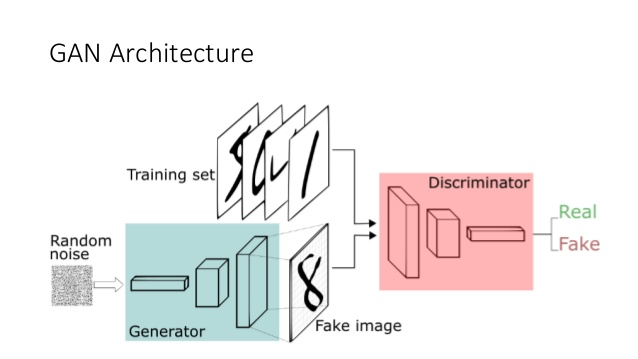
\includegraphics[width=9cm]{gan-arch.jpg}
    \caption{Architecture of a GAN}
    \label{fig:jupyter_server}
\end{figure}


% current state of the art

Since the advent of GANs in 2014, they have vastly improved and have blown up in the AI research field.
State of the art research in GANs is currently focusing at applications in video and voice data. 


\subsection{\label{sec:level2}Applications}

GANs have been applied to many problems \cite{overviewDocument}.\\
A sampling of some of the problems are listed below. 

\begin{itemize}
    \item Image Generation
    \item Music Generation
    \item Style Transfer
    \item Video Prediction
    \item Super Resolution
    \item Text to Image 
\end{itemize}


\subsection{\label{sec:level2}Deep Convolutional Generative Adversarial Network}

Deep Convolutional Generative Adversarial Networks, DCGAN for short, is an architectural modification on the original GAN, in which the generator and discriminator models are reflections of one another.
The makeup of each network is a multi-layer, deep convolutional neural network. The idea behind this architecture is that by reflecting the network structure between the two, the computational capacities of each network to learn their respective tasks is equal \cite{radford2015unsupervised}.
In doing this, it should stabilize competitive learning between the two agents and result in an smoother learning, avoiding cases of one network dominance.


\subsection{\label{sec:level2}Wasserstein Generative Adversarial Networks}

Wasserstein Generative Adversarial Networks, or WGANs for short, were an improvement on the vanilla GAN proposed by Martin Arjovsky, et al in 2017 \cite{arjovsky2017wasserstein}.
The motivation behind this work is modifying the task of the discriminator in order to stabilize the training between the networks. 
Instead of having a simple binary classifier that predicts whether an image is real or fake, the discriminator is modified to output the likelihood estimate of the "realness" or "fakeness" of an image.
The theoretical idea is that this continuous estimation incentivizes the generator to minimize the distance between the distribution of its generated images and the real images more than the standard discriminator design.
Empirically, this design has shown greater results over the standard GAN architecture in terms of training and architecture stability, as well as being more robust to hyper-parameter configurations.

\section{\label{sec:goals}Goals}

% project overview... what we are doing

This project applies three different GAN architectures to generating handwritten images from the MNIST dataset. 
We are going to compare: vanilla GANs, DCGANs, and WGANs.
Using the results of the three different architectures we wish to judge the performance based on three performance criteria:

\begin{itemize}
    \item Perceived Quality of Images
    \item Time required to train
    \item Training data required
\end{itemize}{}

% MNIST data set

The Modified National Institute of Standards and Technology database (MNIST database) is a dataset comprising of seventy thousand handwritten digits.
Sixty thousand of those images are partitioned for training and the remaining ten thousand are left for testing and validation.
We are using the MNIST dataset because it is the de facto standard when it comes to machine learning on images. 


\subsection{\label{sec:level2}Research Questions}

\begin{itemize}
    \item Which GAN architecture performs best on the MNIST dataset?
    \item What are the quantitative differences between these architectures in terms of stability of training, and quality of the results? 
    \item How does required training time and convergence rate differ between GAN architectures?
\end{itemize}

% bibliography via bibtex
\bibliographystyle{ACM-Reference-Format}
\bibliography{proposal}


\end{document}
%
% ****** End of file proposal.tex ******
